% !TeX program = xelatex
\documentclass[a4paper,10pt]{article}

% ============================================================================
% ១. កញ្ចប់បណ្ណាល័យ និងការកំណត់ទំព័រ (Packages & Page Setup — តាមគំរូ ls_plan.tex)
% ============================================================================
\usepackage[a4paper, left=0.95cm, right=0.95cm, top=0.85cm, bottom=0.92cm, footskip=0.52cm]{geometry}
\usepackage{amsmath}
\usepackage{unicode-math}
\usepackage{fontspec}
\usepackage{longtable, array, multirow, colortbl}
\usepackage[table]{xcolor}
\usepackage{enumitem}
\usepackage{pifont}
\usepackage{fancyhdr}
\usepackage{tikz}
\usetikzlibrary{calc, arrows.meta, decorations.pathreplacing, patterns, positioning, babel}

\makeatletter
\let\@expl@@@mark@update@singlecol@structures@@\relax
\makeatother

% --- ប្រព័ន្ធស្វែងរកទីតាំងពុម្ពអក្សរស្វ័យប្រវត្តិ (Windows Local + Cloud Repo fonts/) ---
\providecommand{\NGSFindFonts}{%
  \IfFileExists{C:/Windows/Fonts/cambria.ttc}{%
    \def\NGSSysPath{C:/Windows/Fonts/}%
    \def\NGSUserPath{C:/Users/KIT/AppData/Local/Microsoft/Windows/Fonts/}%
  }{%
    \IfFileExists{./fonts/KhmerOSsiemreap.ttf}{\def\NGSSysPath{./fonts/}\def\NGSUserPath{./fonts/}}{%
    \IfFileExists{../fonts/KhmerOSsiemreap.ttf}{\def\NGSSysPath{../fonts/}\def\NGSUserPath{../fonts/}}{%
    \IfFileExists{../../fonts/KhmerOSsiemreap.ttf}{\def\NGSSysPath{../../fonts/}\def\NGSUserPath{../../fonts/}}{%
    \IfFileExists{../../../fonts/KhmerOSsiemreap.ttf}{\def\NGSSysPath{../../../fonts/}\def\NGSUserPath{../../../fonts/}}{%
    \IfFileExists{../../../../fonts/KhmerOSsiemreap.ttf}{\def\NGSSysPath{../../../../fonts/}\def\NGSUserPath{../../../../fonts/}}{%
    \IfFileExists{../../../../../fonts/KhmerOSsiemreap.ttf}{\def\NGSSysPath{../../../../../fonts/}\def\NGSUserPath{../../../../../fonts/}}{%
    \IfFileExists{../../../../../../fonts/KhmerOSsiemreap.ttf}{\def\NGSSysPath{../../../../../../fonts/}\def\NGSUserPath{../../../../../../fonts/}}{%
      \def\NGSSysPath{../../../../../../../fonts/}\def\NGSUserPath{../../../../../../../fonts/}%
    }}}}}}}%
  }%
}
\NGSFindFonts

% ============================================================================
% ២. កំណត់ពុម្ពអក្សរ (Fonts — តាមគំរូ ls_plan.tex)
% ============================================================================
\setmathfont[Path={\NGSSysPath}, FontIndex=1, Scale=1.02]{cambria.ttc}
\defaultfontfeatures{Ligatures=TeX}

\setmainfont[
  Path={\NGSUserPath},
  Extension=.ttf,
  Script=Khmer,
  BoldFont={KhmerOSsiemreap},
  BoldFeatures={FakeBold=1.8},
  ItalicFont={KhmerOSsiemreap},
  ItalicFeatures={FakeSlant=0.25},
  BoldItalicFont={KhmerOSsiemreap},
  BoldItalicFeatures={FakeBold=1.8, FakeSlant=0.25}
]{KhmerOSsiemreap}

\newfontfamily\muol[Path={\NGSUserPath}, Extension=.ttf, Script=Khmer]{KhmerOSmuollight}
\newfontfamily\Tacteing[Path={\NGSUserPath}, Extension=.TTF]{TACTENG}
\newfontfamily\TimesEn[Path={\NGSSysPath}, Extension=.ttf, BoldFont={timesbd}, ItalicFont={timesi}, BoldItalicFont={timesbi}]{times}
\newfontfamily\CalibriFont[Path={\NGSSysPath}, Extension=.ttf]{calibri}
\newfontfamily\CourierCirc[Path={\NGSSysPath}, Extension=.ttf]{cour}

\XeTeXlinebreaklocale "km"
\XeTeXlinebreakskip = 0pt plus 1pt minus 0.1pt

% ============================================================================
% ៣. ពណ៌ និងការតុបតែង (Colors & Styles)
% ============================================================================
\definecolor{stepbg}{HTML}{D9D9D9}
\definecolor{headgray}{HTML}{E6E6E6}
\definecolor{emphred}{HTML}{C00000}

\pagestyle{fancy}
\fancyhf{}
\renewcommand{\headrulewidth}{0pt}
\fancyfoot[R]{\CalibriFont\fontsize{9pt}{11pt}\selectfont\thepage}

\setlength{\parindent}{0pt}
\setlength{\parskip}{0pt}
\setlength{\tabcolsep}{4.5pt}
\setlength{\LTpre}{2pt}
\setlength{\LTpost}{2pt}

\newcolumntype{L}[1]{>{\raggedright\arraybackslash}p{#1}}
\newcolumntype{C}[1]{>{\centering\arraybackslash}p{#1}}

% ============================================================================
% ៤. ពាក្យបញ្ជាជំនួយ (Helper Macros)
% ============================================================================
\newcommand{\en}[1]{{\TimesEn #1}}
\newcommand{\enbf}[1]{{\TimesEn\bfseries #1}}
\newcommand{\khmflourish}{{\Tacteing\fontsize{15pt}{15pt}\selectfont 3}}
\newcommand{\wcirc}{{\CourierCirc\fontsize{9.5pt}{11pt}\selectfont o}}
\newcommand{\ditem}{{\fontsize{7.5pt}{10pt}\selectfont\ding{117}}\ }
\newcommand{\fiveE}[1]{\textcolor{emphred}{\CalibriFont\bfseries #1}}
\newcommand{\redsub}[1]{\textcolor{emphred}{#1}}
\newcommand{\timenote}[1]{\textcolor{emphred}{\textit{#1}}}
\newcommand{\stepheader}[1]{\multicolumn{3}{|c|}{\cellcolor{stepbg}\muol #1} \\ \hline}
\newcommand{\cfig}[1]{{\centering\vspace{3pt}#1\vspace{3pt}\par}}
\newcommand{\cnum}[1]{\mbox{\fontsize{10.5pt}{12pt}\selectfont\ding{\numexpr181+#1\relax}}}
\newcommand{\unit}[1]{\,\text{\en{#1}}}
\newcommand{\riel}{\,\text{៛}}
\newcommand{\usd}{\,\text{\en{\$}}}
\newcommand{\graybox}[1]{\colorbox{headgray}{\strut #1}}

% ============================================================================
% ៥. រូបភាព TikZ ស-ខ្មៅ សម្រាប់បង្រៀនលើក្ដារខៀន និងសន្លឹកកិច្ចការ (B&W Diagrams)
% ============================================================================

% ១. E1 Engage: បេសកកម្មស្លាកតម្លៃម៉ូតូ 4 000 000៛ (កក់ 1 000 000៛, ការប្រាក់ 10%/ឆ្នាំ, 2 ឆ្នាំ)
\newcommand{\figEngageINSThreeTwoSeven}{%
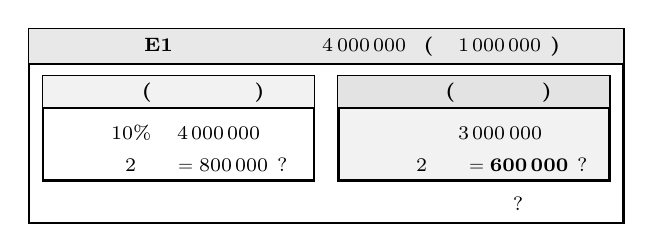
\begin{tikzpicture}[x=1cm, y=1cm, every node/.style={font=\scriptsize, text=black}]
  \draw[black, line width=0.9pt] (0,0) rectangle (7.55,2.46);
  \fill[gray!18] (0,2.02) rectangle (7.55,2.46);
  \draw[black, line width=0.6pt] (0,2.02) -- (7.55,2.02);
  \node at (3.775,2.24) {\textbf{បេសកកម្ម \en{E1}៖ ទិញម៉ូតូបណ្ដាក់ ថ្លៃដើម $4\,000\,000\riel$ (កក់ $1\,000\,000\riel$)}};

  % Left: Buyer A (Misconception)
  \draw[black, line width=0.8pt] (0.18,0.54) rectangle (3.62,1.86);
  \fill[gray!10] (0.18,1.46) rectangle (3.62,1.86);
  \draw[black, line width=0.5pt] (0.18,1.46) -- (3.62,1.46);
  \node at (1.90,1.66) {\textbf{មតិទី ១ (គិតលើថ្លៃដើមទាំងមូល)}};
  \node at (1.90,1.14) {គិត $10\%$ លើ $4\,000\,000\riel$};
  \node at (1.90,0.74) {ការប្រាក់ $2$ ឆ្នាំ $= 800\,000\riel$?};

  % Right: Buyer B (Correct)
  \draw[black, line width=0.95pt, fill=gray!10] (3.93,0.54) rectangle (7.37,1.86);
  \fill[gray!22] (3.93,1.46) rectangle (7.37,1.86);
  \draw[black, line width=0.55pt] (3.93,1.46) -- (7.37,1.46);
  \node at (5.65,1.66) {\textbf{មតិទី ២ (ដកប្រាក់កក់ជាមុន)}};
  \node at (5.65,1.14) {នៅជំពាក់តែ $3\,000\,000\riel$};
  \node at (5.65,0.74) {ការប្រាក់ $2$ ឆ្នាំ $= \mathbf{600\,000\riel}$?};

  \node at (3.775,0.24) {\textbf{សំណួរគន្លឹះ៖} ប្រាក់កក់បង់រួចថ្ងៃដំបូង តើត្រូវគិតការប្រាក់លើវាទៀតដែរឬទេ?};
\end{tikzpicture}}

% ២. E2 Explore: ដ្យាក្រាមលំហូរ ៤ ដំណាក់នៃការទិញកុំព្យូទ័រ (ទំ.៣៨–៣៩ — 9 000 000៛)
\newcommand{\figFlowComputerINSThreeTwoSeven}{%
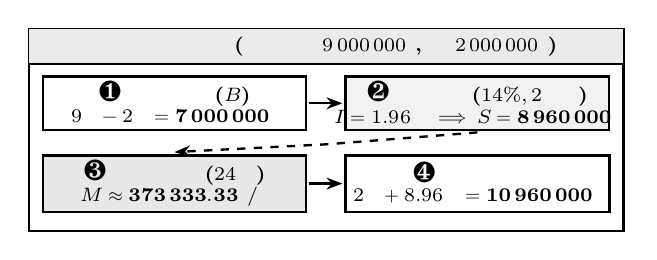
\begin{tikzpicture}[x=1cm, y=1cm, every node/.style={font=\scriptsize, text=black}]
  \draw[black, line width=0.9pt] (0,0) rectangle (7.55,2.56);
  \fill[gray!16] (0,2.12) rectangle (7.55,2.56);
  \draw[black, line width=0.6pt] (0,2.12) -- (7.55,2.12);
  \node at (3.775,2.34) {\textbf{ដ្យាក្រាមលំហូរ ៤ ដំណាក់ (ទិញកុំព្យូទ័រ $9\,000\,000\riel$, កក់ $2\,000\,000\riel$)}};

  % Box 1 & Box 2 (Top row)
  \draw[black, line width=0.8pt] (0.18,1.28) rectangle (3.52,1.96);
  \node at (1.85,1.74) {\textbf{\cnum{1} ប្រាក់នៅជំពាក់ ($B$)}};
  \node at (1.85,1.45) {$9\text{លាន} - 2\text{លាន} = \mathbf{7\,000\,000\riel}$};

  \draw[-{Stealth[length=2mm]}, black, line width=0.85pt] (3.56,1.62) -- (3.98,1.62);

  \draw[black, line width=0.8pt, fill=gray!10] (4.02,1.28) rectangle (7.37,1.96);
  \node at (5.695,1.74) {\textbf{\cnum{2} បូកការប្រាក់ ($14\%, 2$ ឆ្នាំ)}};
  \node at (5.695,1.45) {$I = 1.96\text{លាន} \implies S = \mathbf{8\,960\,000\riel}$};

  % Arrow down to Box 3 & Box 4
  \draw[-{Stealth[length=2mm]}, black, dashed, line width=0.85pt] (5.695,1.25) -- (3.80,1.10) -- (1.85,1.00);

  \draw[black, line width=0.95pt, fill=gray!18] (0.18,0.24) rectangle (3.52,0.96);
  \node at (1.85,0.74) {\textbf{\cnum{3} សងរំលស់ប្រចាំខែ ($24$ ខែ)}};
  \node at (1.85,0.44) {$M \approx \mathbf{373\,333.33\riel}$/ខែ};

  \draw[-{Stealth[length=2mm]}, black, line width=0.85pt] (3.56,0.60) -- (3.98,0.60);

  \draw[black, line width=0.95pt] (4.02,0.24) rectangle (7.37,0.96);
  \node at (5.695,0.74) {\textbf{\cnum{4} ថ្លៃទិញបណ្ដាក់សរុប}};
  \node at (5.695,0.44) {$2\text{លាន} + 8.96\text{លាន} = \mathbf{10\,960\,000\riel}$};
\end{tikzpicture}}

% ៣. E3 Explain: ប្រៀបធៀបថ្លៃលក់មិនបណ្ដាក់ ទល់នឹង ថ្លៃទិញបណ្ដាក់សរុប
\newcommand{\figBarCompareINSThreeTwoSeven}{%
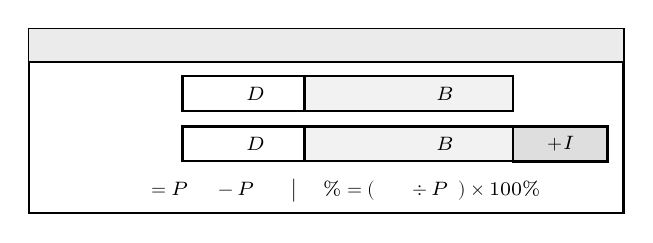
\begin{tikzpicture}[x=1cm, y=1cm, every node/.style={font=\scriptsize, text=black}]
  \draw[black, line width=0.9pt] (0,0) rectangle (7.55,2.34);
  \fill[gray!16] (0,1.92) rectangle (7.55,2.34);
  \draw[black, line width=0.6pt] (0,1.92) -- (7.55,1.92);
  \node at (3.775,2.13) {\textbf{រចនាសម្ព័ន្ធថ្លៃទិញមិនបណ្ដាក់ ទល់នឹង ថ្លៃទិញបណ្ដាក់សរុប}};

  % Cash price bar
  \node[anchor=west] at (0.18,1.52) {\textbf{មិនបណ្ដាក់៖}};
  \draw[black, line width=0.8pt] (1.95,1.30) rectangle (3.50,1.74);
  \node at (2.725,1.52) {កក់ $D$};
  \draw[black, line width=0.8pt, fill=gray!10] (3.50,1.30) rectangle (6.15,1.74);
  \node at (4.825,1.52) {ប្រាក់ជំពាក់ $B$};

  % Hire-purchase bar
  \node[anchor=west] at (0.18,0.88) {\textbf{ទិញបណ្ដាក់៖}};
  \draw[black, line width=0.8pt] (1.95,0.66) rectangle (3.50,1.10);
  \node at (2.725,0.88) {កក់ $D$};
  \draw[black, line width=0.8pt, fill=gray!10] (3.50,0.66) rectangle (6.15,1.10);
  \node at (4.825,0.88) {ប្រាក់ជំពាក់ $B$};
  \draw[black, line width=0.95pt, fill=gray!26] (6.15,0.66) rectangle (7.35,1.10);
  \node at (6.75,0.88) {$+I$};

  \node at (3.775,0.28) {បន្ថែម $= P_{\text{បណ្ដាក់}} - P_{\text{ដើម}}$ \quad $\big|$ \quad $\% = (\text{បន្ថែម} \div P_{\text{ដើម}})\times 100\%$};
\end{tikzpicture}}

% ៤. E4 Elaborate: លំហាត់គំរូទី១ ម៉ាស៊ីនបោកខោអាវ (ទំ.៣៩ — 1 350 000៛, កក់ 15%, 10 2/3%, 2 ឆ្នាំ)
\newcommand{\figWasherModelINSThreeTwoSeven}{%
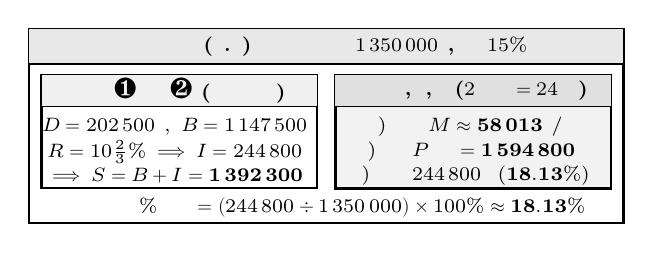
\begin{tikzpicture}[x=1cm, y=1cm, every node/.style={font=\scriptsize, text=black}]
  \draw[black, line width=0.9pt] (0,0) rectangle (7.55,2.46);
  \fill[gray!18] (0,2.02) rectangle (7.55,2.46);
  \draw[black, line width=0.6pt] (0,2.02) -- (7.55,2.02);
  \node at (3.775,2.24) {\textbf{លំហាត់គំរូទី១ (ទំ.៣៩)៖ ម៉ាស៊ីនបោកខោអាវ $1\,350\,000\riel$, កក់ $15\%$}};

  % Left box
  \draw[black, line width=0.8pt] (0.16,0.44) rectangle (3.66,1.88);
  \fill[gray!12] (0.16,1.48) rectangle (3.66,1.88);
  \draw[black, line width=0.55pt] (0.16,1.48) -- (3.66,1.48);
  \node at (1.91,1.68) {\textbf{ដំណាក់ \cnum{1} និង \cnum{2} (ប្រាក់ជំពាក់)}};
  \node at (1.91,1.22) {$D = 202\,500\riel, \ B = 1\,147\,500\riel$};
  \node at (1.91,0.90) {$R = 10\tfrac{2}{3}\% \implies I = 244\,800\riel$};
  \node at (1.91,0.60) {$\implies S = B + I = \mathbf{1\,392\,300\riel}$};

  % Right box
  \draw[black, line width=0.95pt, fill=gray!10] (3.89,0.44) rectangle (7.39,1.88);
  \fill[gray!24] (3.89,1.48) rectangle (7.39,1.88);
  \draw[black, line width=0.6pt] (3.89,1.48) -- (7.39,1.48);
  \node at (5.64,1.68) {\textbf{ចម្លើយ ក, ខ, គ ($2\text{ ឆ្នាំ} = 24\text{ ខែ}$)}};
  \node at (5.64,1.22) {ក) រំលស់ $M \approx \mathbf{58\,013\riel}$/ខែ};
  \node at (5.64,0.90) {ខ) សរុប $P_{\text{បណ្ដាក់}} = \mathbf{1\,594\,800\riel}$};
  \node at (5.64,0.60) {គ) សន្សំ $244\,800\riel$ ($\mathbf{18.13\%}$)};

  \node at (3.775,0.20) {ផ្ទៀងផ្ទាត់៖ $\% \text{ សន្សំ} = (244\,800 \div 1\,350\,000)\times 100\% \approx \mathbf{18.13\%}$};
\end{tikzpicture}}

% ៥. E5 Evaluate: ជម្រើសវិនិច្ឆ័យ A-D (ទិញកង់ ថ្លៃដើម 600 000៛, កក់ 100 000៛, រំលស់ 62 000៛ x 10 ខែ)
\newcommand{\figExitINSThreeTwoSeven}{%
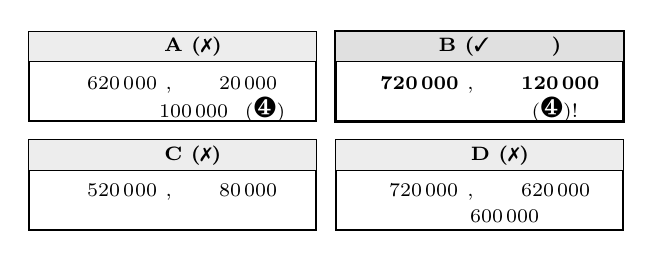
\begin{tikzpicture}[x=1cm, y=1cm, every node/.style={font=\scriptsize, text=black}]
  % Choice A
  \draw[black, line width=0.8pt] (0,1.38) rectangle (3.65,2.52);
  \fill[gray!14] (0,2.14) rectangle (3.65,2.52);
  \draw[black, line width=0.5pt] (0,2.14) -- (3.65,2.14);
  \node at (1.825,2.33) {\textbf{ជម្រើស \en{A} (\ding{55})}};
  \node at (1.825,1.84) {សរុប $620\,000\riel$, បន្ថែម $20\,000\riel$};
  \node at (1.825,1.53) {ភ្លេចបូកប្រាក់កក់ $100\,000\riel$ (\cnum{4})};

  % Choice B (Correct)
  \draw[black, line width=1.05pt] (3.90,1.38) rectangle (7.55,2.52);
  \fill[gray!24] (3.90,2.14) rectangle (7.55,2.52);
  \draw[black, line width=0.6pt] (3.90,2.14) -- (7.55,2.14);
  \node at (5.725,2.33) {\textbf{ជម្រើស \en{B} (\ding{51} ត្រឹមត្រូវ)}};
  \node at (5.725,1.84) {សរុប $\mathbf{720\,000\riel}$, បន្ថែម $\mathbf{120\,000\riel}$};
  \node at (5.725,1.53) {បូកប្រាក់កក់ និងរំលស់ត្រូវ (\cnum{4})!};

  % Choice C
  \draw[black, line width=0.8pt] (0,0) rectangle (3.65,1.14);
  \fill[gray!14] (0,0.76) rectangle (3.65,1.14);
  \draw[black, line width=0.5pt] (0,0.76) -- (3.65,0.76);
  \node at (1.825,0.95) {\textbf{ជម្រើស \en{C} (\ding{55})}};
  \node at (1.825,0.48) {សរុប $520\,000\riel$, បន្ថែម $80\,000\riel$};
  \node at (1.825,0.18) {ច្រឡំដកប្រាក់កក់ចេញពីប្រាក់រំលស់};

  % Choice D
  \draw[black, line width=0.8pt] (3.90,0) rectangle (7.55,1.14);
  \fill[gray!14] (3.90,0.76) rectangle (7.55,1.14);
  \draw[black, line width=0.5pt] (3.90,0.76) -- (7.55,0.76);
  \node at (5.725,0.95) {\textbf{ជម្រើស \en{D} (\ding{55})}};
  \node at (5.725,0.48) {សរុប $720\,000\riel$, បន្ថែម $620\,000\riel$};
  \node at (5.725,0.18) {ភ្លេចដកថ្លៃដើម $600\,000\riel$ ចេញ};
\end{tikzpicture}}

\begin{document}
\fontsize{10pt}{15.2pt}\selectfont

% ============================================================================
% ក្បាលរដ្ឋបាល (Administrative Header — តាមគំរូ ls_plan.tex)
% ============================================================================
{\centering
  {\muol\fontsize{11pt}{16pt}\selectfont ព្រះរាជាណាចក្រកម្ពុជា\par}
  {\muol\fontsize{11pt}{16pt}\selectfont ជាតិ សាសនា ព្រះមហាក្សត្រ\par}
  \vspace{-3pt}{\khmflourish\par}
}

\vspace{1pt}
{\muol\fontsize{10pt}{15.5pt}\selectfont
មន្ទីរអប់រំ យុវជន និងកីឡា ខេត្តកំពង់ធំ\par
ការិយាល័យអប់រំ យុវជន និងកីឡា ស្រុកកំពង់ស្វាយ\par
អនុវិទ្យាល័យព្រះក្រសាំង\par}

\vspace{4pt}
{\centering{\muol\fontsize{11.5pt}{17pt}\selectfont កិច្ចតែងការបង្រៀន\par}}
\vspace{3pt}

% --- ព័ត៌មានទូទៅ ---
{\hspace*{2.8cm}\renewcommand{\arraystretch}{1.08}
\begin{tabular}{@{}l@{\hspace{0.35cm}}p{2.9cm}@{\hspace{0.15cm}}c@{\hspace{0.25cm}}l@{}}
  - & មុខវិជ្ជា & : & គណិតវិទ្យា ថ្នាក់ទី៨ (ពីជគណិត) \\
  - & ចំណងជើងមេរៀន & : & មេរៀនទី៣៖ ទំហំសមាមាត្រនិងភាគរយ \\
  - & ចំណងជើងរង & : & ២.៧. ការទិញបណ្ដាក់ (ទំ.៣៨--៤០, ៤២) \\
  - & រយៈពេល & : & ១ ម៉ោងសិក្សា (៥០ នាទី) \\
  - & បង្រៀនដោយ & : & ហុក ប៊ុនថែន \\
  - & កាលបរិច្ឆេទ & : & ថ្ងៃព្រហស្បតិ៍ ទី២៦ ខែវិច្ឆិកា ឆ្នាំ២០២៦ \\
\end{tabular}\par}

\vspace{4pt}

% --- I. វត្ថុបំណង ---
{\muol\fontsize{10pt}{15.5pt}\selectfont \enbf{I.} វត្ថុបំណង\par}
\vspace{1pt}
{\renewcommand{\arraystretch}{1.10}
\begin{tabular}{@{}p{0.55cm}@{}p{2.35cm}@{\hspace{0.15cm}}c@{\hspace{0.25cm}}p{14.95cm}@{}}
  \hfill\wcirc\hspace{0.2cm} & វិជ្ជាសម្បទា & : & សិស្សប្រាប់និយមន័យនៃការទិញបណ្ដាក់ ប្រាក់កក់ ប្រាក់នៅជំពាក់ ប្រាក់សងរំលស់ប្រចាំខែ ថ្លៃទិញបណ្ដាក់សរុប និងលក្ខខណ្ឌកម្មសិទ្ធិលើទំនិញបានត្រឹមត្រូវ ។ \\
  \hfill\wcirc\hspace{0.2cm} & បំណិនសម្បទា & : & សិស្សគណនាប្រាក់នៅជំពាក់ ការប្រាក់ ប្រាក់សងរំលស់ប្រចាំខែ ថ្លៃទិញបណ្ដាក់សរុប និងភាគរយប្រាក់បន្ថែមធៀបនឹងថ្លៃលក់មិនបណ្ដាក់ តាមដ្យាក្រាមលំហូរ ៤ ដំណាក់លើសន្លឹកកិច្ចការ (ទំ.៣៨--៤០) បានត្រឹមត្រូវ ។ \\
  \hfill\wcirc\hspace{0.2cm} & ចរិយាសម្បទា & : & សិស្សមានទម្លាប់ប្រៀបធៀបថ្លៃទិញបណ្ដាក់និងថ្លៃទិញមិនបណ្ដាក់មុនសម្រេចចិត្តទិញសម្ភារៈប្រើប្រាស់ក្នុងគ្រួសារប្រកបដោយការទទួលខុសត្រូវផ្នែកហិរញ្ញវត្ថុ ។ \\
\end{tabular}\par}

\vspace{3pt}

% --- II. សម្ភារៈឧបទេស ---
{\muol\fontsize{10pt}{15.5pt}\selectfont \enbf{II.} សម្ភារៈឧបទេស\par}
\vspace{1pt}
\hspace*{0.55cm}$\bullet$\ សៀវភៅសិក្សាគោលថ្នាក់ទី៨ (ទំ.៣៨--៤០, ៤២) ក្ដារខៀន ដីស/ហ្វឺត បន្ទាត់ត្រង់ និង\textbf{សន្លឹកកិច្ចការសិស្សបំពេញចន្លោះ ស-ខ្មៅ} (\en{Printable\_Materials\_INS327} ទំព័រ ១--២ សម្រាប់សិស្ស និងទំព័រ ៣ ប្លង់ក្ដារខៀន/ចម្លើយគ្រូ — គ្មានប្រើ \en{LCD})\par

\vspace{3pt}

% --- III. វិធីសាស្រ្តបង្រៀន ---
{\muol\fontsize{10pt}{15.5pt}\selectfont \enbf{III.} វិធីសាស្រ្តបង្រៀន\par}
\vspace{1pt}
{\renewcommand{\arraystretch}{1.08}
\begin{tabular}{@{}p{0.55cm}@{}p{2.35cm}@{\hspace{0.15cm}}c@{\hspace{0.25cm}}p{14.95cm}@{}}
  \hfill$\bullet$\hspace{0.2cm} & គោលវិធី & : & សិស្សមជ្ឈមណ្ឌល (សន្លឹកកិច្ចការបំពេញចន្លោះជាគោល + ការពិភាក្សាជាក្រុមតូច ៣ នាក់) \\
  \hfill$\bullet$\hspace{0.2cm} & យុទ្ធវិធីបង្រៀន & : & គំរូស្ថាបនានិយម \en{5Es} រួមបញ្ចូល \textbf{ដ្យាក្រាមលំហូរ ៤ ដំណាក់នៃការទិញបណ្ដាក់} និង \textbf{ការប្រៀបធៀបថ្លៃមិនបណ្ដាក់ ទល់នឹង ថ្លៃបណ្ដាក់} \\
\end{tabular}\par}

\vspace{3pt}

% --- IV. ដំណើរការបង្រៀន ---
{\muol\fontsize{10pt}{15.5pt}\selectfont \enbf{IV.} ដំណើរការបង្រៀន\par}

{\renewcommand{\arraystretch}{1.15}
\begin{longtable}{|L{5.50cm}|L{7.90cm}|L{4.80cm}|}
\hline
\multicolumn{1}{|c|}{\cellcolor{headgray}\muol សកម្មភាពគ្រូ} &
\multicolumn{1}{c|}{\cellcolor{headgray}\muol ខ្លឹមសារមេរៀន} &
\multicolumn{1}{c|}{\cellcolor{headgray}\muol សកម្មភាពសិស្ស} \\
\hline
\endfirsthead

\hline
\multicolumn{1}{|c|}{\cellcolor{headgray}\muol សកម្មភាពគ្រូ} &
\multicolumn{1}{c|}{\cellcolor{headgray}\muol ខ្លឹមសារមេរៀន} &
\multicolumn{1}{c|}{\cellcolor{headgray}\muol សកម្មភាពសិស្ស} \\
\hline
\endhead

% ==================== ជំហានទី១ (2min) ====================
\stepheader{ជំហានទី១ \enbf{(}រដ្ឋបាលថ្នាក់\enbf{)}}
$\bullet$ ពិនិត្យវត្តមាន អនាម័យ និងសណ្ដាប់ធ្នាប់ថ្នាក់រៀន \par
$\bullet$ រៀបចំក្រុមតូច ៣ នាក់តាមតុ និងចែក\textbf{សន្លឹកកិច្ចការសិស្ស (\en{INS327} ទំព័រ ១–២)}
&
$\bullet$ រដ្ឋបាលថ្នាក់ អនាម័យ និងវិន័យសិក្សា \par
$\bullet$ ចែកសន្លឹកកិច្ចការម្នាក់ ១ សន្លឹក សម្រាប់បំពេញតាមដំណាក់កាល \en{E1--E5}
&
$\circ$ ប្រធានថ្នាក់រាយការណ៍វត្តមានសិស្ស \par
$\circ$ ទទួលសន្លឹកកិច្ចការ សរសេរឈ្មោះ និងអង្គុយតាមក្រុម ៣ នាក់ \\
\hline

% ==================== ជំហានទី២ (9min: កំណែ <=3m + រំលឹក 3m + E1 3m) ====================
\stepheader{ជំហានទី២ \enbf{(}កិច្ចការផ្ទះ \enbf{+} ទំនាក់ទំនងមេរៀនថ្មី\enbf{)}}
\ditem \textbf{កំណែកិច្ចការផ្ទះ ($\le\text{\enbf{3\,min}}$)} \par
$\bullet$ ហៅសិស្ស ២ នាក់ឡើងកែលំហាត់ទំ.៤២ លេខ ១៧(ក,ខ) និងលេខ ១៨ លើក្ដារខៀន
&
{\centering\redsub{កំណែកិច្ចការផ្ទះមេរៀនមុន (ទំ.៤២ \#17 ក,ខ និង \#18)}\par}
$\bullet$ \textbf{\#17 (ទំ.៤២)៖} (ក) $1\,800\,000\riel, 2$ ឆ្នាំ, $10\% \implies I_{\text{សមាស}} = \mathbf{378\,000\riel}$; (ខ) $2\,800\,000\riel, 3$ ឆ្នាំ, $11\% \implies I_{\text{សមាស}} = \mathbf{1\,029\,366.8\riel}$ \par
$\bullet$ \textbf{\#18 (ទំ.៤២ — ពូសឿន)៖} ប្រាក់សរុបដំណាច់ឆ្នាំទី៣ $A_3 = \mathbf{30\,417\,500\riel}$
&
$\circ$ ផ្ទៀងចម្លើយ និងកែតម្រូវចូលសៀវភៅកិច្ចការផ្ទះ \\[3pt]

\ditem \textbf{រំលឹកមេរៀនទាក់ទង (\enbf{3min})} \par
$\bullet$ សួរ៖ «រូបមន្តការប្រាក់សាមញ្ញសរសេរដូចម្ដេច? ហើយ $2$ ឆ្នាំ ត្រូវនឹងប៉ុន្មានខែ?»
&
{\centering\redsub{រំលឹកការប្រាក់សាមញ្ញ និងការបំប្លែងឆ្នាំ-ខែ}\par}
$\bullet$ ការប្រាក់សាមញ្ញ៖ $I = \tfrac{P\times R\times T}{100}$ ($T$ គិតជាឆ្នាំ)
&
$\circ$ ឆ្លើយ៖ «$I = \frac{PRT}{100}$ ហើយ $2$ ឆ្នាំ $= 24$ ខែ!» \\[3pt]

$\bullet$ សួរបន្ត៖ «ចុះបើសងរំលស់ $48$ ខែ តើត្រូវនឹងប៉ុន្មានឆ្នាំ?»
&
$\bullet$ បំប្លែងខែជាឆ្នាំ៖ $24\text{ ខែ} = 2\text{ ឆ្នាំ}$, \quad $48\text{ ខែ} = \tfrac{48}{12} = 4\text{ ឆ្នាំ}$
&
$\circ$ ឆ្លើយ៖ «$48$ ខែ ត្រូវនឹង $4$ ឆ្នាំ!» \\[3pt]

\fiveE{E1 - Engage (3min)} \timenote{(កុំទាន់ផ្ដល់ចម្លើយ)} \par
\ditem \textbf{បេសកកម្មស្លាកតម្លៃម៉ូតូបណ្ដាក់ (សន្លឹកកិច្ចការ \en{E1})} \par
$\bullet$ ឱ្យសិស្សអានប្រអប់ \en{E1} ហើយគូសជ្រើសរើសរវាង\textbf{មតិទី ១} និង\textbf{មតិទី ២}
&
\redsub{បេសកកម្ម \en{E1}៖ ទិញម៉ូតូបណ្ដាក់ ថ្លៃដើម $4\,000\,000\riel$ (កក់មុន $1\,000\,000\riel$)} \par
ហាងលក់ម៉ូតូមួយកំណត់ថ្លៃលក់មិនបណ្ដាក់ $4\,000\,000\riel$ ឬទិញបណ្ដាក់ដោយកក់មុន $1\,000\,000\riel$ ហើយបង់ការប្រាក់ $10\%$/ឆ្នាំ រយៈពេល $2$ ឆ្នាំ ($24$ ខែ) ។ \par
$\bullet$ តើហាងត្រូវគិតការប្រាក់លើ $4\,000\,000\riel$ ឬគិតតែលើប្រាក់នៅជំពាក់ $3\,000\,000\riel$?
&
$\circ$ ពិភាក្សាជាគូ និងគូស \ding{51} ក្នុងប្រអប់ \en{E1} លើសន្លឹកកិច្ចការ \\[3pt]

&
\cfig{\figEngageINSThreeTwoSeven}
& \\
\hline

% ==================== ជំហានទី៣ (17min: E2 11m + E3 6m) ====================
\stepheader{ជំហានទី៣ \enbf{(}ខ្លឹមសារមេរៀនថ្មី\enbf{)}}
\fiveE{E2 - Explore (11min)} \par
$\bullet$ សរសេរចំណងជើងរង \textbf{២.៧. ការទិញបណ្ដាក់} លើក្ដារខៀន \par
\ditem \textbf{សកម្មភាព ១៖ ដ្យាក្រាមលំហូរ ៤ ដំណាក់នៃការទិញកុំព្យូទ័រ (\enbf{6min}, សន្លឹកកិច្ចការ \en{E2-A})} \par
$\bullet$ ឱ្យសិស្សបំពេញប្រអប់ទាំង ៤ នៃឧទាហរណ៍ទិញកុំព្យូទ័រ (សៀវភៅទំ.៣៨–៣៩)
&
មេរៀនទី៣ \quad {\muol ទំហំសមាមាត្រនិងភាគរយ \enbf{(}ត\enbf{)}} \par
២.៧. ការទិញបណ្ដាក់ \par
$\bullet$ \textbf{ឧទាហរណ៍ (ទំ.៣៨–៣៩ — ទិញកុំព្យូទ័រ $9\,000\,000\riel$, កក់ $2\,000\,000\riel$, $R=14\%$, $2$ ឆ្នាំ)៖} \par
\hspace*{0.2cm}-- \textbf{ដំណាក់ \cnum{1} ប្រាក់នៅជំពាក់៖} $B = 9\,000\,000 - 2\,000\,000 = \mathbf{7\,000\,000\riel}$ \par
\hspace*{0.2cm}-- \textbf{ដំណាក់ \cnum{2} ការប្រាក់ $2$ ឆ្នាំ៖} $I = \dfrac{7\,000\,000\times 14\times 2}{100} = \mathbf{1\,960\,000\riel}$ \par
\hspace*{0.45cm}$\implies$ ប្រាក់នៅជំពាក់បូកការប្រាក់ $S = 7\,000\,000 + 1\,960\,000 = \mathbf{8\,960\,000\riel}$ \par
\hspace*{0.2cm}-- \textbf{ដំណាក់ \cnum{3} ប្រាក់សងរំលស់ប្រចាំខែ ($24$ ខែ)៖} $M = \dfrac{8\,960\,000}{24} \approx \mathbf{373\,333.33\riel}$
&
$\circ$ បំពេញដ្យាក្រាមលំហូរលើសន្លឹកកិច្ចការ \en{E2-A} ឃើញប្រាក់រំលស់ $373\,333.33\riel$/ខែ \\[3pt]

&
\cfig{\figFlowComputerINSThreeTwoSeven}
& \\[3pt]

\ditem \textbf{សកម្មភាព ២៖ អន្ទាក់ភ្លេចដកប្រាក់កក់ និងថ្លៃទិញបណ្ដាក់សរុប (\enbf{5min}, សន្លឹកកិច្ចការ \en{E2-B})} \par
$\bullet$ សួរ៖ «បើភ្លេចដកប្រាក់កក់ $2\,000\,000\riel$ តើខុសការប្រាក់ប៉ុន្មាន? ហើយថ្លៃទិញបណ្ដាក់សរុបស្មើប៉ុន្មាន?»
&
$\bullet$ \textbf{ពិនិត្យអន្ទាក់ និងថ្លៃទិញបណ្ដាក់សរុប (ដំណាក់ \cnum{4})៖} \par
\hspace*{0.2cm}-- បើច្រឡំគិតការប្រាក់លើ $9\,000\,000\riel$ នោះ $I = 2\,520\,000\riel$ (\textbf{ខុស! លើស $560\,000\riel$}) \par
\hspace*{0.2cm}-- \textbf{ថ្លៃទិញបណ្ដាក់សរុប៖} $P_{\text{បណ្ដាក់}} = 2\,000\,000 + 8\,960\,000 = \mathbf{10\,960\,000\riel}$ \par
\hspace*{0.2cm}-- \textbf{កម្មសិទ្ធិ (ទំ.៣៨)៖} អ្នកទិញក្លាយជាម្ចាស់កម្មសិទ្ធិពេញលេញ លុះត្រាតែសងរំលស់អស់!
&
$\circ$ រកឃើញថាការប្រាក់គិតតែលើប្រាក់នៅជំពាក់ ហើយថ្លៃបណ្ដាក់សរុបស្មើ $10\,960\,000\riel$ \\[3pt]

% --- E3 Explain (6min) ---
\fiveE{E3 - Explain (6min)} \par
$\bullet$ ដឹកនាំសិស្សសង្ខេបរូបមន្តគោលនៃ\textbf{ការទិញបណ្ដាក់} (ទំ.៣៨–៣៩)
&
$\bullet$ \textbf{ក្បួនគណនាការទិញបណ្ដាក់ (ទំ.៣៨–៣៩)៖} \par
\hspace*{0.15cm}១) ប្រាក់នៅជំពាក់៖ \graybox{$B = P_{\text{ដើម}} - D$} \quad ២) ប្រាក់សងរំលស់សរុប៖ \graybox{$S = B + I$}
&
$\circ$ បំពេញប្រអប់រូបមន្តលើសន្លឹកកិច្ចការ \en{E3} \\[3pt]

$\bullet$ កត់ត្រារូបមន្តប្រាក់សងរំលស់ប្រចាំខែ និងថ្លៃទិញបណ្ដាក់សរុប
&
\hspace*{0.15cm}៣) សងរំលស់ប្រចាំខែ ($m$ ខែ)៖ \graybox{$M = \dfrac{S}{m}$} \quad ៤) ថ្លៃបណ្ដាក់សរុប៖ \graybox{$P_{\text{បណ្ដាក់}} = D + S = D + m\times M$}
&
$\circ$ កត់ត្រារូបមន្ត $M$ និង $P_{\text{បណ្ដាក់}}$ លើសន្លឹកកិច្ចការ \en{E3} \\[3pt]

&
\cfig{\figBarCompareINSThreeTwoSeven}
& \\[3pt]

$\bullet$ ភ្ជាប់\textbf{ធនាគារហេតុផល \cnum{1}--\cnum{4}} លើក្ដារខៀន និងសន្លឹកកិច្ចការ
&
\textbf{ធនាគារហេតុផល (\en{Warrant Bank})៖} \par
\cnum{1} \textbf{ដកប្រាក់កក់ជាមុន៖} គិតការប្រាក់តែលើប្រាក់នៅជំពាក់ $B = P_{\text{ដើម}} - D$ \par
\cnum{2} \textbf{ការប្រាក់លើប្រាក់ជំពាក់៖} $I = \frac{B\times R\times T}{100}$ ($T$ គិតជាឆ្នាំ) រួច $S = B + I$ \par
\cnum{3} \textbf{សងរំលស់ប្រចាំខែ៖} ចែក $S$ នឹង\textbf{ចំនួនខែសរុប $m$} ($M = \frac{S}{m}$) \par
\cnum{4} \textbf{ថ្លៃបណ្ដាក់សរុប និង $\%$ បន្ថែម៖} $P_{\text{បណ្ដាក់}} = D + S$; $\% = \frac{P_{\text{បណ្ដាក់}} - P_{\text{ដើម}}}{P_{\text{ដើម}}}\times 100\%$
&
$\circ$ ផ្ទៀងលេខកូដ \cnum{1}--\cnum{4} លើសន្លឹកកិច្ចការ \\
\hline

% ==================== ជំហានទី៤ (20min: E4 10m + E5 10m) ====================
\stepheader{ជំហានទី៤ \enbf{(}ពង្រីកចំណេះដឹង\enbf{)}}
\fiveE{E4 - Elaborate (10min)} \par
\ditem \textbf{លំហាត់គំរូទី ១៖ ម៉ាស៊ីនបោកខោអាវ ទំ.៣៩} \par
$\bullet$ ឱ្យសិស្សបំពេញដំណាក់ \cnum{1}--\cnum{4} សម្រាប់ម៉ាស៊ីនបោកខោអាវ ($1\,350\,000\riel$, កក់ $15\%$, អត្រា $10\frac{2}{3}\%$, $2$ ឆ្នាំ) លើសន្លឹកកិច្ចការ \en{E4}
&
{\muol លំហាត់គំរូទី ១} \textbf{(ទំ.៣៩ — ថ្លៃដើម $1\,350\,000\riel$, កក់ $15\%$, $R = 10\frac{2}{3}\% = \frac{32}{3}\%$, $2$ ឆ្នាំ)៖} \par
$\bullet$ ប្រាក់កក់ $D = \frac{15}{100}\times 1\,350\,000 = 202\,500\riel \implies B = 1\,350\,000 - 202\,500 = 1\,147\,500\riel$ (\cnum{1}) \par
$\bullet$ ការប្រាក់ $I = 1\,147\,500\times \frac{32}{3}\times \frac{1}{100}\times 2 = 244\,800\riel \implies S = 1\,392\,300\riel$ (\cnum{2}) \par
$\bullet$ \textbf{ក) សងរំលស់ប្រចាំខែ ($24$ ខែ)៖} $M = \frac{1\,392\,300}{24} = 58\,012.5\riel \approx \graybox{$58\,013\riel$}$ (\cnum{3}) \par
$\bullet$ \textbf{ខ) ថ្លៃទិញបណ្ដាក់សរុប៖} $P_{\text{បណ្ដាក់}} = 202\,500 + 1\,392\,300 = \graybox{$1\,594\,800\riel$}$ (\cnum{4}) \par
$\bullet$ \textbf{គ) ប្រាក់សន្សំបើទិញមិនបណ្ដាក់៖} $244\,800\riel \implies \frac{244\,800}{1\,350\,000}\times 100\% = \graybox{$18\frac{2}{15}\% \approx 18.13\%$}$
&
$\circ$ បំប្លែង $10\frac{2}{3}\% = \frac{32}{3}\%$ និងគណនាចម្លើយ ក, ខ, គ លើសន្លឹកកិច្ចការ \en{E4} \\[3pt]

&
\cfig{\figWasherModelINSThreeTwoSeven}
& \\[3pt]

$\bullet$ សួរសំណួរឆ្លុះបញ្ចាំង \textbf{\en{EIA Looking-Back} (1min)}
&
\textbf{\en{EIA Looking-Back}៖} «បើគេប្រាប់ប្រាក់សងរំលស់ប្រចាំខែ $M$ និងចំនួនខែ $m$ ស្រាប់ តើយើងរកថ្លៃទិញបណ្ដាក់សរុបតាមរូបមន្តណា?» ($\to$ តាម $P_{\text{បណ្ដាក់}} = D + m\times M$ ដោយមិនបាច់រកអត្រាការប្រាក់ឡើយ!)
&
$\circ$ ឆ្លើយភ្ជាប់ទៅតារាងប្រតិបត្តិ $P_{\text{បណ្ដាក់}} = D + m\times M$ \\[3pt]

% --- E5 Evaluate (10min) ---
\fiveE{E5 - Evaluate (10min)} \par
\ditem \textbf{ប្រតិបត្តិជាក្រុមតូច ៣ នាក់ (4min, សន្លឹកកិច្ចការ \en{E5})}
&
{\muol លំហាត់ប្រតិបត្តិ} \textbf{(ទំ.៤០ — រកប្រាក់បន្ថែម និងភាគរយនៃថ្លៃមិនបណ្ដាក់)៖}
&
$\circ$ អានតារាងប្រតិបត្តិ (ក និង ខ) លើសន្លឹកកិច្ចការ \en{E5} \\[3pt]

$\bullet$ ឱ្យសិស្សគណនាជួរ (ក) តាមរូបមន្ត \cnum{4}
&
$\bullet$ \textbf{ក)} $P_{\text{ដើម}} = 1\,080\,000\riel$, $D = 150\,000\riel$, រំលស់ $120\,000\riel \times 10$ ខែ $\implies P_{\text{បណ្ដាក់}} = 1\,350\,000\riel \implies$ បន្ថែម $\mathbf{270\,000\riel}$ ($\mathbf{25\%}$)
&
$\circ$ គណនាជួរ (ក) ឃើញបន្ថែម $270\,000\riel$ ត្រូវនឹង $25\%$ \\[3pt]

$\bullet$ ត្រួតពិនិត្យជួរ (ខ) តាមធនាគារហេតុផល \cnum{4}
&
$\bullet$ \textbf{ខ)} $P_{\text{ដើម}} = 2\,700\,000\riel$, $D = 450\,000\riel$, រំលស់ $225\,000\riel \times 12$ ខែ $\implies P_{\text{បណ្ដាក់}} = 3\,150\,000\riel \implies$ បន្ថែម $\mathbf{450\,000\riel}$ ($\mathbf{16\frac{2}{3}\% \approx 16.67\%}$)
&
$\circ$ គណនាជួរ (ខ) ឃើញបន្ថែម $450\,000\riel$ ត្រូវនឹង $16\frac{2}{3}\%$ \\[3pt]

$\bullet$ ឱ្យក្រុមសិស្សផ្ទៀងផ្ទាត់និង\textbf{បិទបេសកកម្ម \en{E1} (2min)}
&
$\bullet$ \textbf{បិទបេសកកម្ម \en{E1}៖} មតិទី ២ ត្រឹមត្រូវ! $B = 3\,000\,000\riel \implies I = \frac{3\,000\,000\times 10\times 2}{100} = \mathbf{600\,000\riel} \implies S = 3\,600\,000\riel \implies M = \mathbf{150\,000\riel}$/ខែ ។
&
$\circ$ បិទបេសកកម្ម \en{E1} ឃើញមតិទី ២ ត្រឹមត្រូវ ($M = 150\,000\riel$/ខែ) \\[3pt]

\ditem \textbf{សំណួរវិនិច្ឆ័យ \en{A--D} និងសំបុត្រចេញ (4min)} \par
$\bullet$ ឱ្យសិស្សគូសរង្វង់ជម្រើសត្រូវលើសន្លឹកកិច្ចការ រួចលើកម្រាមដៃ ១--៤
&
{\centering\textbf{សំណួរវិនិច្ឆ័យ \en{A--D}៖ ទិញកង់ថ្លៃដើម $600\,000\riel$ កក់មុន $100\,000\riel$ និងបង់រំលស់ $62\,000\riel$/ខែ ចំនួន $10$ ខែ ។ រកថ្លៃបណ្ដាក់សរុប និងប្រាក់បន្ថែម ៖}\par}
&
$\circ$ វិភាគជម្រើស \en{A--D} និងលើកម្រាមដៃ ២ (\textbf{ជម្រើស \en{B}}) \\[3pt]

&
\cfig{\figExitINSThreeTwoSeven}
& \\[3pt]

$\bullet$ បញ្ជាក់ចម្លើយត្រូវ (\textbf{ជម្រើស \en{B}}) និងឱ្យបំពេញ\textbf{សំបុត្រចេញ ៦០ វិនាទី}
&
$\bullet$ \textbf{សំបុត្រចេញ៖} ទូរស័ព្ទថ្លៃដើម $800\,000\riel$ កក់ $200\,000\riel$ ការប្រាក់ $10\%$/ឆ្នាំ រយៈពេល $1$ ឆ្នាំ ($12$ ខែ) $\implies B = \mathbf{600\,000\riel}$, $I = \mathbf{60\,000\riel}$, $M = \mathbf{55\,000\riel}$/ខែ, $P_{\text{បណ្ដាក់}} = \mathbf{860\,000\riel}$ ។
&
$\circ$ បំពេញសំបុត្រចេញលើសន្លឹកកិច្ចការមុនបញ្ចប់ម៉ោង \\
\hline

% ==================== ជំហានទី៥ (<=2min) ====================
\stepheader{ជំហានទី៥ \enbf{(}កិច្ចការផ្ទះ \enbf{+} បណ្ដាំផ្ញើ\enbf{)}}
\timenote{ចំណាយពេលឱ្យតិចបំផុតកុំឱ្យលើស 2min} \par
$\bullet$ ណែនាំប្រអប់\textbf{កិច្ចការផ្ទះ}លើសន្លឹកកិច្ចការទំព័រ ២ (លំហាត់ទំ.៤២ លេខ ១៩ ក, ខ)
&
{\centering{\muol កិច្ចការផ្ទះ} \textbf{(សៀវភៅគោល ទំ.៤២ លេខ ១៩ ក និង ខ)}\par} \par
$\bullet$ \textbf{\#19 (ទំ.៤២ — ពូគាទិញម៉ាស៊ីនត្រជាក់ $2\,700\,000\riel$, កក់ $20\%$, រំលស់ $48$ ខែ, $R=10\%$/ឆ្នាំ)៖} \par
\hspace*{0.2cm}(ក) រកប្រាក់សងរំលស់ប្រចាំខែ ($\to \mathbf{63\,000\riel}$/ខែ); (ខ) រកប្រាក់សន្សំបានបើទិញមិនជំពាក់ ($\to \mathbf{864\,000\riel}$) ។
&
$\circ$ គូសចំណាំលំហាត់ \#19(ក,ខ) ទំ.៤២ \\[3pt]

$\bullet$ ណែនាំការបំប្លែង $48\text{ ខែ} = 4\text{ ឆ្នាំ}$ និងផ្ដាំផ្ញើអានមេរៀនទី៤ បន្ទាប់
&
$\bullet$ \textbf{បណ្ដាំផ្ញើ៖} អានមុន \textbf{មេរៀនទី៤៖ រង្វាស់រង្វាល់ — ១. ផ្ទៃក្រឡានិងមាឌ (ទំ.៤៣–៤៤)} សម្រាប់ម៉ោងក្រោយ ។
&
$\circ$ កត់ត្រាបណ្ដាំផ្ញើ ទុកសន្លឹកកិច្ចការក្នុងសៀវភៅ និងជម្រាបលាគ្រូ \\
\hline
\end{longtable}}

\vspace{6pt}
% --- ហត្ថលេខា (កាលបរិច្ឆេទត្រូវគ្នា ១០០% នឹងខាងលើ) ---
{\centering
\hspace*{5.2cm}\begin{minipage}{11.5cm}
  \centering
  ថ្ងៃព្រហស្បតិ៍ ២រោច ខែកត្តិក ឆ្នាំមមី អដ្ឋស័ក ពុទ្ធសករាជ ២៥៧០\par
  កំពង់ស្វាយ, ថ្ងៃទី២៦ ខែវិច្ឆិកា ឆ្នាំ២០២៦\par
  \vspace{2pt}
  {\muol គ្រូបង្រៀន\par}
  \vspace{32pt}
  \hfill{\muol ហុក ប៊ុនថែន}\hspace*{1.4cm}
\end{minipage}\par}

\end{document}
